\chapter{Literature Review}
\label{ch:review}
\vspace{2em}

In this chapter, we introduce the literature support used for this project. To start with, we first review some of the latest studies about vessel trajectory prediction. We further explain in more detail about the AIS message and the underlying end-to-end system behind data collection and generation of the AIS data. We also review the theoretical work in the field of recurrent neural network and one of its archetypes for handling sequential data.

\section{Trajectory Prediction Model}
This section will review some of the latest works on the trajectory prediction model using the AIS dataset. The trajectory prediction model is essentially a model to predict the future movement of a vessel given its historic navigation information.

Hexeberg \emph{et al.} \cite{hexeberg2017ais} uses the nearest neighbor search method to predict the future of a vessel's course and speed based on historical AIS data. Nearest Neighbors Search seeks to optimize the closest neighbors for a given coordinate measured with Harvesine Distance metrics. The algorithm shows good potential for vessel trajectory prediction up to about 30 minutes ahead and can follow paths of various curvatures. However, when the trajectory is too tight in the event of branching or turning, the predicted position fails to follow the same path. This could be fixed by reducing the step length and time step duration.

Young \cite{young2017predicting} builds a random forest and neural network model to predict the future position of a vessel at a given timestep based on the clustered routes of AIS data. He clusters similar trajectories of the vessel and uses collective information about a route from all ships belong to the same cluster to determine the next position of the vessel. He found out that random forest outperforms neural network in all regions in datasets, that random forest shows better accuracy, simpler and faster to run than the neural network.

Liraz \cite{liraz2018ships} develops vessel trajectory prediction models with a Recurrent Neural Network (RNN) architecture called Long Short Term Memory (LSTM). She uses LSTM to learn the Spatio-temporal dependency of AIS data and conclude that the best way to predict vessel location is to build a model with a fixed multi timestep interval into the future as opposed to short single time step forward prediction. Neural network models in general work best with adding more data and tuning some of their hyper-parameters.

\section{Automatic Identification System (AIS)}
AIS is a transponder system designed to be capable of exchanging information between ships and between ships to coastal authorities. In 2004, the International Maritime Organization enacted Regulation 19 of SOLAS Chapter V about ship-borne navigational systems and equipment. The regulation requires every ship of 300 gross tonnages upwards and engaged in international voyage or passenger vessel irrespective of its size to be installed with AIS devices on board. Ships that equipped with the AIS transceiver device shall transmit the following information in 3 categories 1). fixed information, including MMSI number, IMO number, call sign, and type of ship. 2). dynamic information, including ship's position, position time stamps, course over ground (COG), speed over ground (SOG), and heading direction. 3). voyage information, including ship's draught, hazardous cargo, destination and estimated time arrival (ETA), and route plan. AIS messages are broadcast by transponders on ships and stations by Very High-Frequency radio (VHF) periodically. AIS messages are received by VHF receivers on other ships or stations within the frequency band range. The typical AIS message is transmitted in a form as shown in Table~\ref{tab:ais_table}:

\begin{table}[ht]
\caption{Encoded version of AIS message}
\label{tab:ais_table}
\centering
\begin{tabular}{|c||c|}
\hline
Type & Message\\
\hline
Encoded & !AIVDM,1,1,,B,B8HsgOP001ne@DP;uP@03wnTkP06,0*5F\\
\hline
\end{tabular}
\end{table}

\section{AIS Data Collection System}
The School of Computing at the National University of Singapore designed and implemented an end-to-end solution for AIS data collection, cleaning, and generation and made them publicly available in \url{www.data.liancheng.science}. The complete apparatus of the system consists of 5 parts: 
\begin{itemize}
    \item VHF antenna to receive the AIS message in binary format.
    \item GPS antenna to receive ship's current position.
    \item Devices called AIS receiver connected to both antennas.
    \item Web server called ``ais-receiver'' responsible for displaying the ship on a map in real-time.
    \item Web server called ``neptune'' responsible for publishing the decoded AIS message logs in JavaScript Object Notation (JSON) format every month.
\end{itemize}

At the beginning of the process, AIS message is received by the AIS receiver device connected to both antennas in binary/encoded format as shown in Table \ref{tab:ais_table}. The next machine connected to the first receiver via USB is responsible for performing 3 tasks. \textit{First}, reading the message from the first receiver through a C++ program that reads the stream of the message, logs them to the hard drive, and dispatch them in real-time over the network. \textit{Second}, monitoring the ships via a service called ``navigator'', a small light Sinatra web framework written in Ruby language to display the ship's navigation using Google Map in real-time. It decodes information necessary to display the location on the map such as longitude, latitude, course, and type of vessel. Currently ``navigator'' uses NUS Open ID for authentication, which means it can only be accessed with NUS account. For future development, ``navigator'' will be set up with Nginx as a reverse proxy for better concurrency performance. \textit{Third}, archiving the message logs via a service called ``cron'', a Ruby script run once a month which does a set of actions for the AIS message logs from history. The ``cron'' service essentially perform following actions: 
\begin{itemize}
    \item archives the AIS binary logs, which typically consist of the starting time of the record, GPS location, single-line message, multiple line messages, invalid messages,
    \item pre-process the binary logs by filtering invalid messages and noise, and output the result in JSON format,
    \item count the messages in the archives and updates the ship's database,
    \item store the ship information into open source database platform PostgreSQL on a yearly basis.
\end{itemize}
The last machine in the system is called ``neptune'', a web service that connects to ``ais-machine'' through TCP/IP socket such that allows them to access all archives of AIS message and make them available on the web in \url{www.data.liancheng.science}. The web page is refreshed once a month by running a ruby script that copies all archives from ``ais-machine'' to ``neptune'' and generating a new static HTML to display the new archived files. 

\section{Artificial Neural Network}
Artificial Neural Network has recently become a powerful tool to perform machine-learning related tasks using image, text, and audio data. Artificial Neural Network is a model computation inspired by the structured of neural networks in the brain. In a much-simplified version of the brain, it consists of many computing devices (neuron) that are interconnected, through which the brain can carry out highly complex computation \cite{shwartzdavid2014}. A simplified version of neuron is called \emph{perceptron}, and we will discuss the mechanics of perceptron to understand more complex neural network. Perceptrons were developed in the 1950s by scientist Frank Rosenbaltt. A perceptron takes multiple binary input and produce a single binary output. Suppose perceptrons takes several input $x_1$, $x_2$, and $x_3$ and output $y$. Rosenbaltt propose a simple rule to compute the output by introducing \emph{weights} denoted as $w_1$, $w_2$, ..., a real numbers expressing the importance of each input; the higher the value, the more important the input is \cite{nielsenneural}. The output $y$ is computed by multiplying each input with the corresponding weight. Mathematically it is expressed as $y$ = $w_1$ $x_1$ + $w_2$ $x_2$ + ... + $w_i$ $x_i$. The perceptron output is either 0 or 1 depending on whether the output $y$ is less or greater than certain tresshold. Perceptrons ``know'' the value of its \emph{weights} from fitting the input, or sometimes referred as training. Usually they do not get the most accurate \emph{weights} in the first shot as it starts-off with random value. As the perceptrons learn the pattern of input and output, eventually they get the \emph{weights} approximately correct. Coming back to discussion of neuron, a nueron is simply a version of perceptron with an activation function in its output. Activation function, just like any function, defines the output given its input.

From the single perceptron, we can build a larger networks consist of multiple perceptrons and even multiple layers. In fact, there exist such network named Multiple Layers Perceptrons (MLP). The term ``layers'' literally means the layer of network whereby the first layer takes the input from data, the second layer takes the output from the first layer as the input, and so on, until the last layer can only produce an output. The following MLP in Figure \ref{fig:mlp} has 4 layers with two of them are hidden layers. We can add more layers and neurons depending on how complex the data is. A common practice would be to start building a simple network with small layers and see the performance. Then we can decide to add or even reduce the network complexity accordingly.

\begin{figure}[t!]
    \centering
    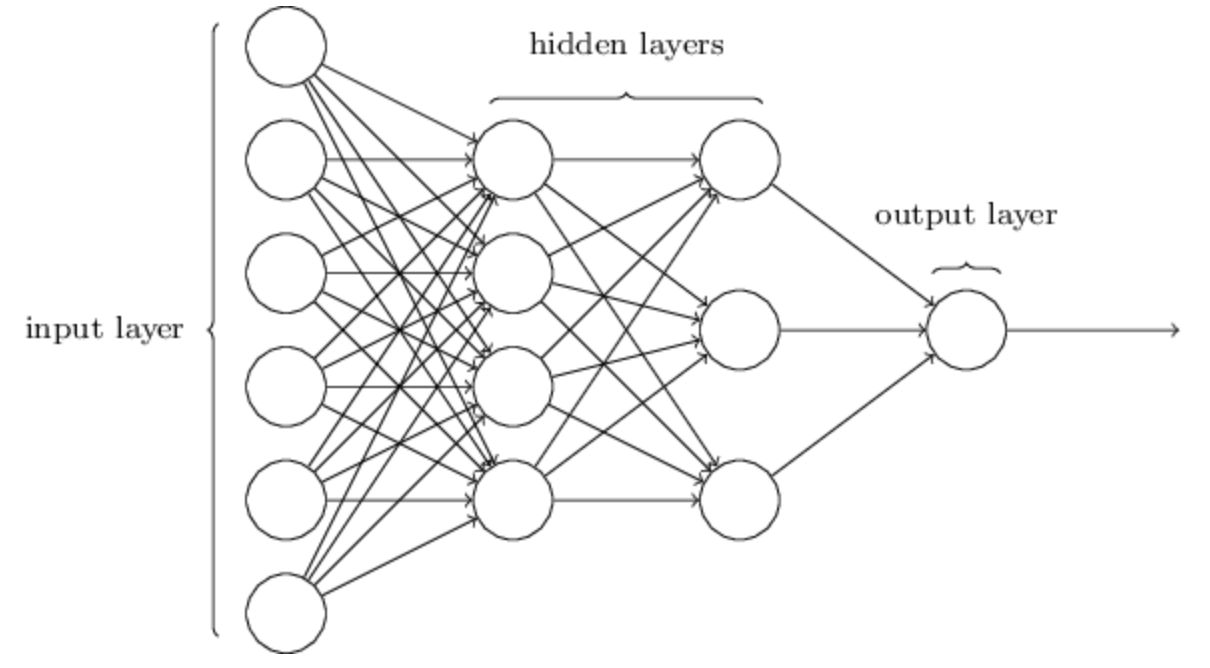
\includegraphics[width=10cm]{pic/ch-review/mlp.png}
    \caption{Multi layer perceptron with 4 layers and 2 hidden layers. Picture taken from Neural Networks and Deep Learning, Michael Nielson}
    \label{fig:mlp}
\end{figure}

\subsection{Recurrent Neural Network (RNN)}
The standard neural network we have discussed previously failed to address the fact that human brain process a sequence information like sentence by understanding the previous words or even previous sentences. Sequence data could be text or any data that have time dependency. In other words, there is need for another version of neural network to remember the context of previous sequence while iterating through the next sequence. Recurrent Neural Network exactly address this issue. RNN is a network with internal loop allowing the information to persist. The network is presented in Figure \ref{fig:rnn-rolled}.

\begin{figure}[t!]
    \centering
    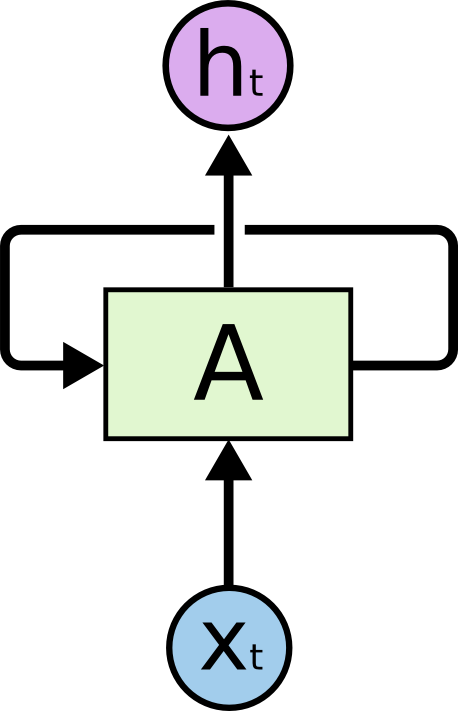
\includegraphics[width=2cm]{pic/ch-review/RNN-rolled.png}
    \caption{RNN network with internal loop. Picture taken from Chris Olah}
    \label{fig:rnn-rolled}
\end{figure}

\begin{figure}[t!]
    \centering
    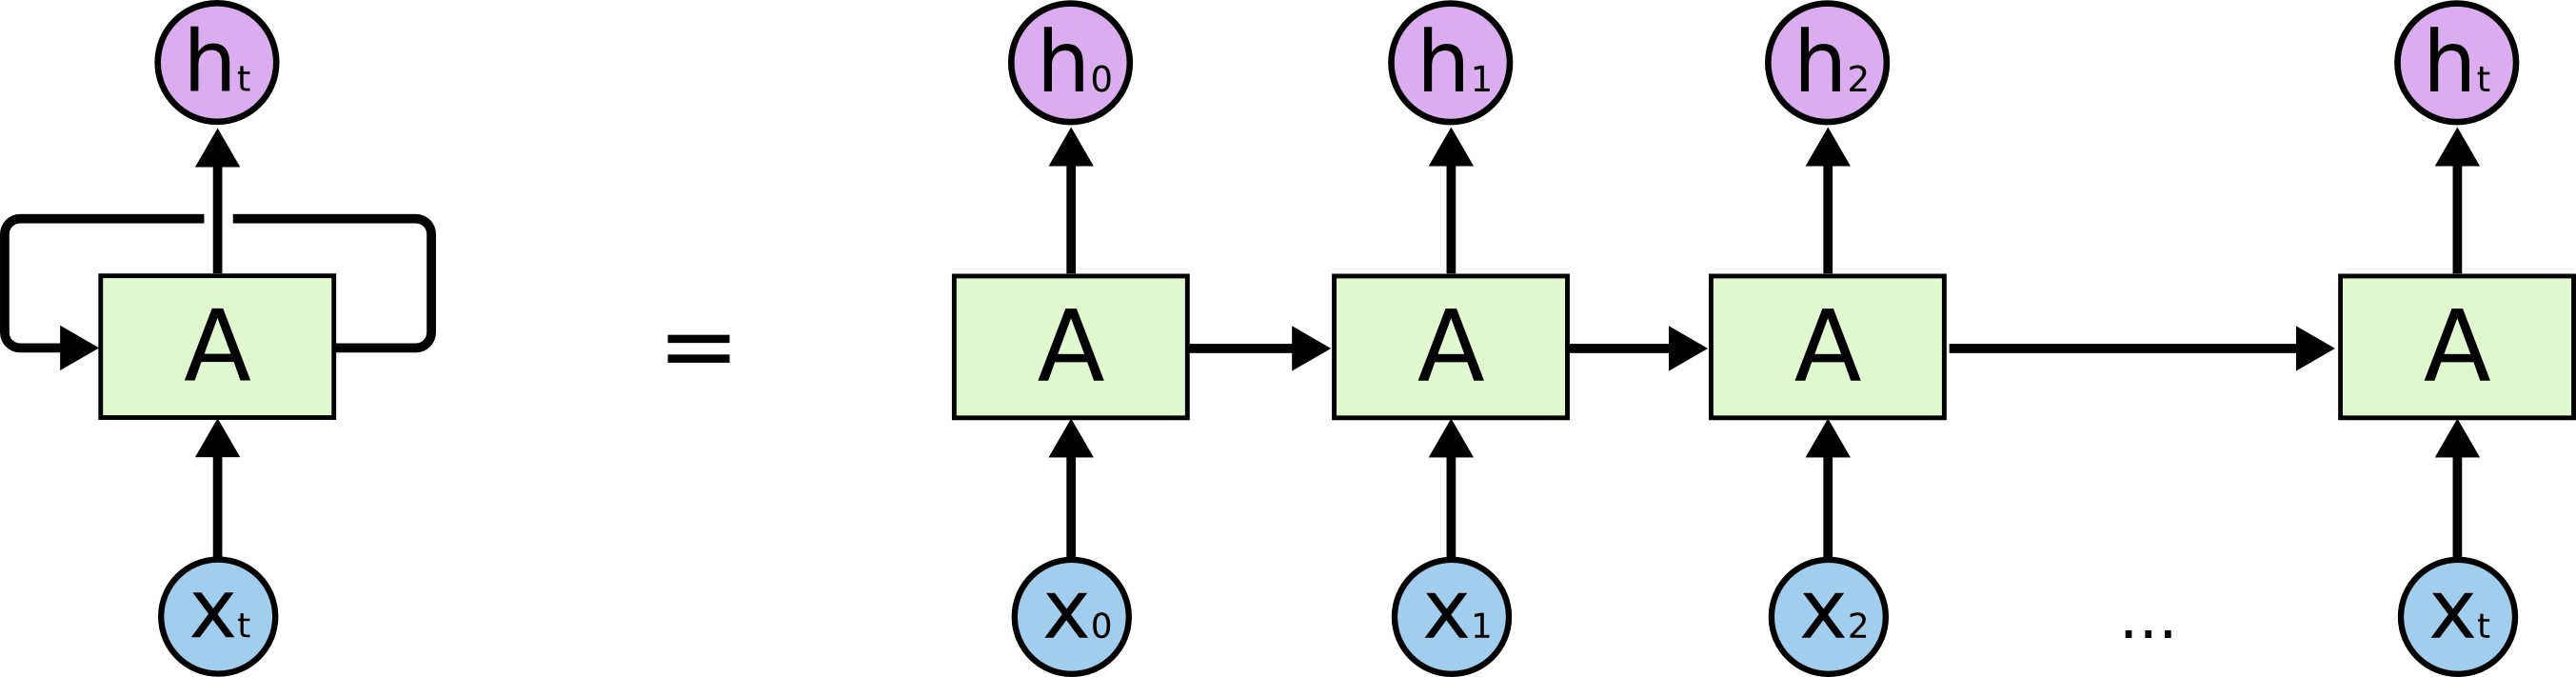
\includegraphics[width=10cm]{pic/ch-review/RNN-unrolled.png}
    \caption{RNN network processing sequence of input. Picture taken from Chris Olah}
    \label{fig:rnn-unrolled}
\end{figure}

Figure \ref{fig:rnn-unrolled} is how the RNN process the sequence of input represented by $x_0$, $x_1$, $x_2$, ... $x_t$ and have output of $y_0$, $y_1$, $y_2$, ... $y_t$. The network process sequence data by iterating thorough the sequence elements and maintaining a \emph{state} containing information relative to what it has seen so far \cite{franoischollet2017learning}. RNN has been useful to solve many problems including language modelling, image captioning, and translation. However there is problem with the performance. RNN have difficulty in remembering information from a long time ago. It could be failure to remember specific information in the first sentence of the paragraph while processing the last sentence. RNN is also known to be computationally expensive.

Long Short Term Memory (LSTM) come to solve the long term dependency problem that RNN have a hard time with in practice. LSTM was introduced first time by Hochreiter \& Schmidhuber in 1997, and improved over the years by many studies. LSTM is specifically designed to remember long term information by introducing new node called \emph{gates}. The core principle of LSTM is still similar to the standard RNN, they are just different in the internal mechanics of single network. 

\begin{figure}[t!]
    \centering
    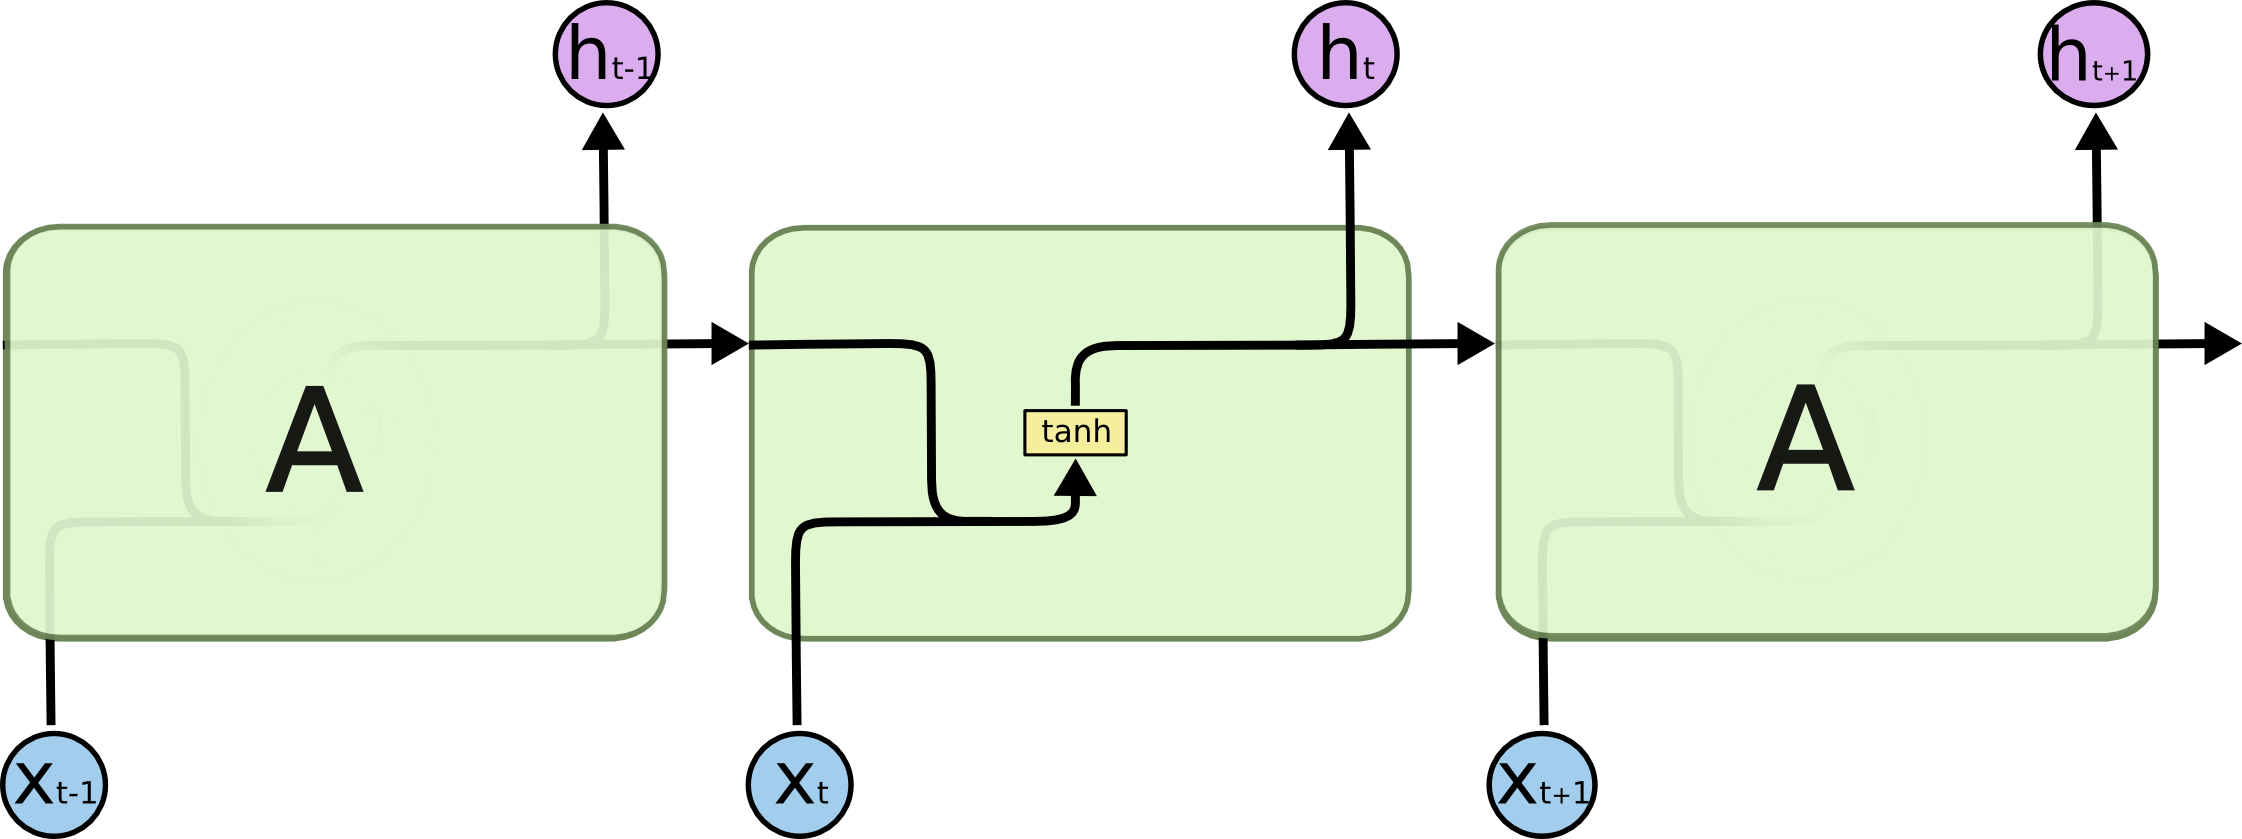
\includegraphics[width=10cm]{pic/ch-review/LSTM3-SimpleRNN.png}
    \caption{Standard RNN internal mechanichsm. Picture taken from Chris Olah}
    \label{fig:rnn}
\end{figure}

\begin{figure}[t!]
    \centering
    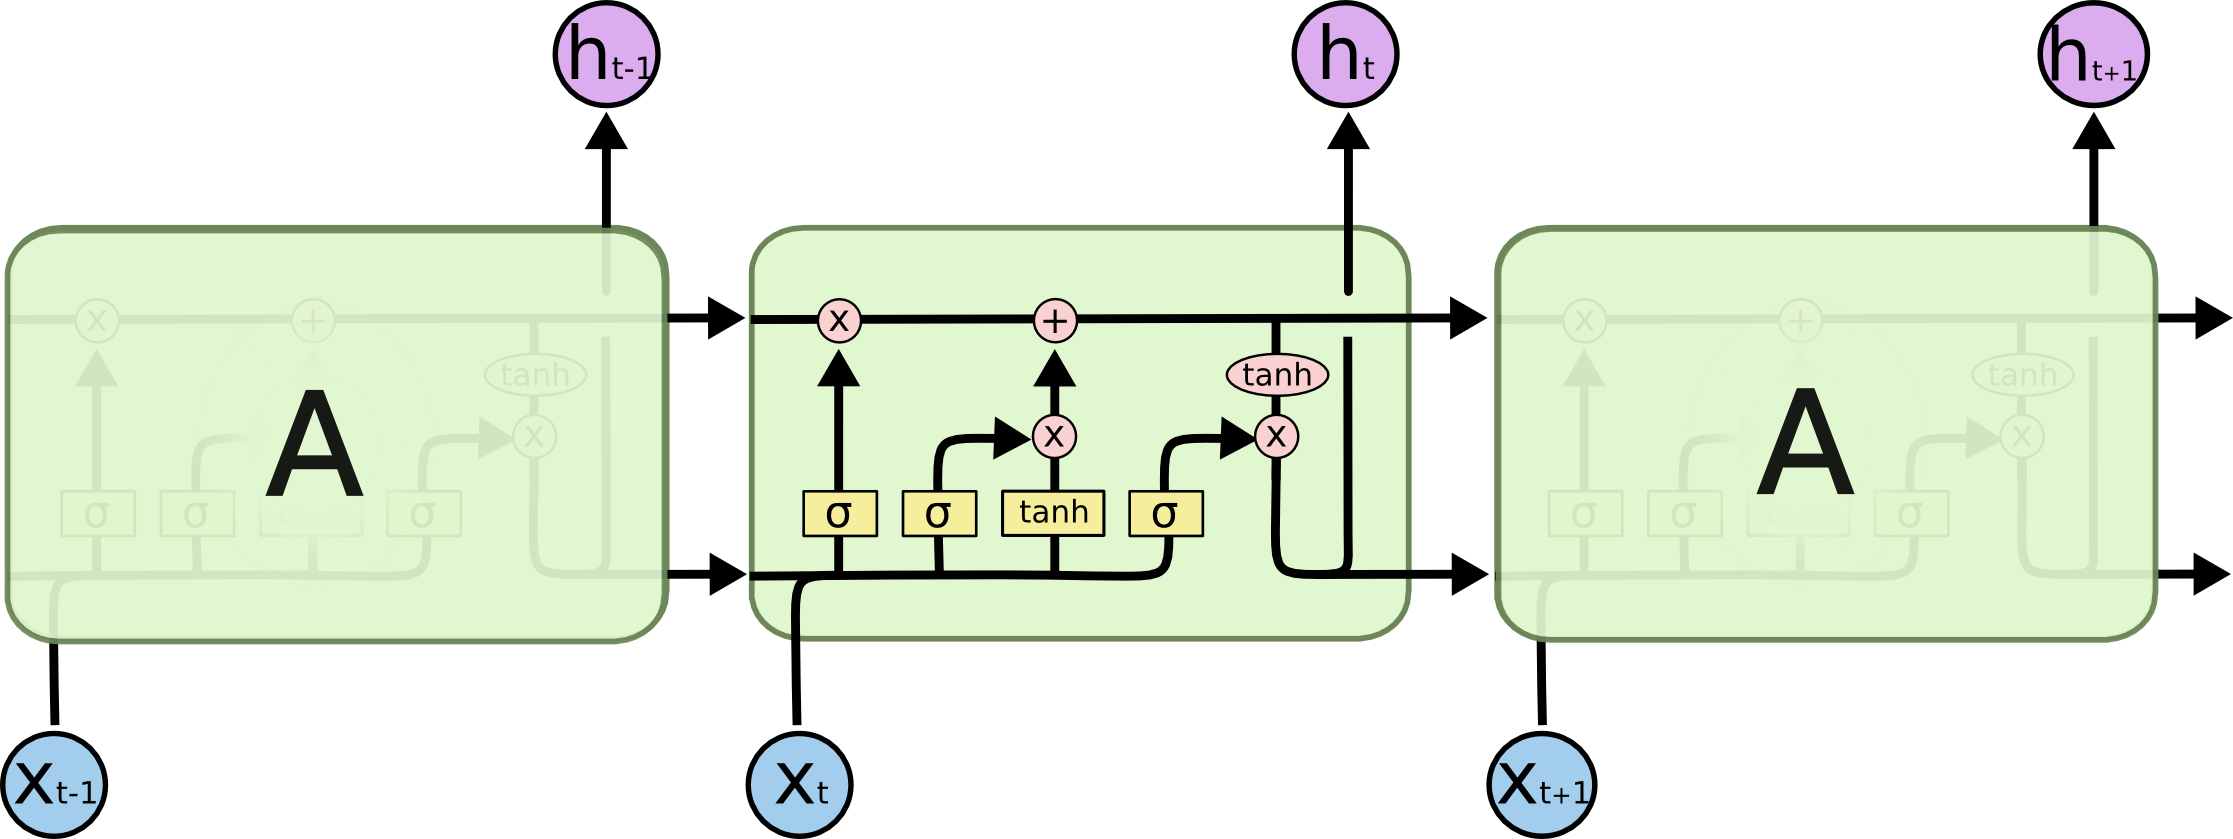
\includegraphics[width=10cm]{pic/ch-review/LSTM3-chain.png}
    \caption{LSTM, an improved version of RNN introduce new node called gates. Picture taken from Chris Olah}
    \label{fig:lstm}
\end{figure}

There we see in Figure \ref{fig:lstm}, the \emph{gates} node was introduced with sigmoid function and pointwise multiplication. The purpose of the gates is to decide which information to ``forget'' or pass depending on the output of sigmoid activation function. A value of zero means ``let nothing through'' and a value of one means ``let everything through'' \cite{lstmcolah}. The gate act like information regulator which evaluate the importance of information to let through to the next cell.